% The Slide Definitions
%document
\documentclass[10pt]{beamer}
%theme
\usetheme{metropolis}
% packages
\usepackage{color}
\usepackage{listings}
\usepackage[ngerman]{babel}
\usepackage[utf8]{inputenc}
\usepackage{multicol}


% color definitions
\definecolor{mygreen}{rgb}{0,0.6,0}
\definecolor{mygray}{rgb}{0.5,0.5,0.5}
\definecolor{mymauve}{rgb}{0.58,0,0.82}

\lstset{
    backgroundcolor=\color{white},
    % choose the background color;
    % you must add \usepackage{color} or \usepackage{xcolor}
    basicstyle=\footnotesize\ttfamily,
    % the size of the fonts that are used for the code
    breakatwhitespace=false,
    % sets if automatic breaks should only happen at whitespace
    breaklines=true,                 % sets automatic line breaking
    captionpos=b,                    % sets the caption-position to bottom
    commentstyle=\color{mygreen},    % comment style
    % deletekeywords={...},
    % if you want to delete keywords from the given language
    extendedchars=true,
    % lets you use non-ASCII characters;
    % for 8-bits encodings only, does not work with UTF-8
    frame=single,                    % adds a frame around the code
    keepspaces=true,
    % keeps spaces in text,
    % useful for keeping indentation of code
    % (possibly needs columns=flexible)
    keywordstyle=\color{blue},       % keyword style
    % morekeywords={*,...},
    % if you want to add more keywords to the set
    numbers=left,
    % where to put the line-numbers; possible values are (none, left, right)
    numbersep=5pt,
    % how far the line-numbers are from the code
    numberstyle=\tiny\color{mygray},
    % the style that is used for the line-numbers
    rulecolor=\color{black},
    % if not set, the frame-color may be changed on line-breaks
    % within not-black text (e.g. comments (green here))
    stepnumber=1,
    % the step between two line-numbers.
    % If it's 1, each line will be numbered
    stringstyle=\color{mymauve},     % string literal style
    tabsize=4,                       % sets default tabsize to 4 spaces
    % show the filename of files included with \lstinputlisting;
    % also try caption instead of title
    language = Python,
	showspaces = false,
	showtabs = false,
	showstringspaces = false,
	escapechar = ,
}

\def\ContinueLineNumber{\lstset{firstnumber=last}}
\def\StartLineAt#1{\lstset{firstnumber=#1}}
\let\numberLineAt\StartLineAt



\newcommand{\codeline}[1]{
	\alert{\texttt{#1}}
}


% Author and Course information
% This Document contains the information about this course.

% Authors of the slides
\author{Claas de Boer, Tilman Hinnerichs}

% Name of the Course
\institute{Python-Grundlagen}

% Fancy Logo 
\titlegraphic{\hfill
\includegraphics[height=1.25cm]{../images/fsr_logo_cropped}}

% Custom Bindings
% \newcommand{\codeline}[1]{
%	\alert{\texttt{#1}}
%}


% Presentation title
\title{Allgemeine Informationen}
\date{12.11.2020}

\begin{document}
	
\maketitle

\begin{frame}{Gliederung}
	\setbeamertemplate{section in toc}[sections numbered]
	\tableofcontents
\end{frame}

\section{Allgemeine Informationen}
\begin{frame}{Anforderungen}
	Ihr müsst...
	\begin{itemize}
		\item einen Computer bedienen können
		\item eigenständig Python 3.x installieren
		\item keine weiteren Programmierkenntnisse haben
	\end{itemize}
\end{frame}

\begin{frame}{Some resources}
	Falls ihr Hilfe braucht...
	\begin{itemize}
		\item fragt uns oder eure Komillitonen
		\item besucht StackOverflow, FAQs, Onlinetutorials, $\dots$
		\item studiert die offizielle Doku unter \hfill \\
			\url{https://docs.python.org/3/}
		\item schaut euch noch einmal die Folien an unter \hfill \\
			\url{https://github.com/THinnerichs/python-beginner-lessons}
	\end{itemize}
\end{frame}

\section{Kursablauf}
\begin{frame}{Wie wird der Kurs ablaufen?}
	
	Ablauf:
	\begin{itemize}
		\item Es wird 11 Sessions geben
		\item Jede einzelne wird ein anderes Thema behandeln
	\end{itemize}

	\pause
	\begin{itemize}
		\item Sessions in BigBlueButton: https://bbb.agdsn.de/til-jq7-kyn
		\item Ein Interpreter + Entwicklungsumgebung eurer Wahl:
		\begin{itemize}
			\item Präferiert: Vanilla Python Shell oder IDE eurer Wahl
			\item Ansonsten: \url{https://repl.it/languages/Python3}
		\end{itemize}
		\item Gruppenarbeiten in Unterräumen und Codesharing über \url{codeshare.io}
	\end{itemize}	
\end{frame}

\section{Warum Python?}
\begin{frame}{Warum Python?}
	\begin{figure}
		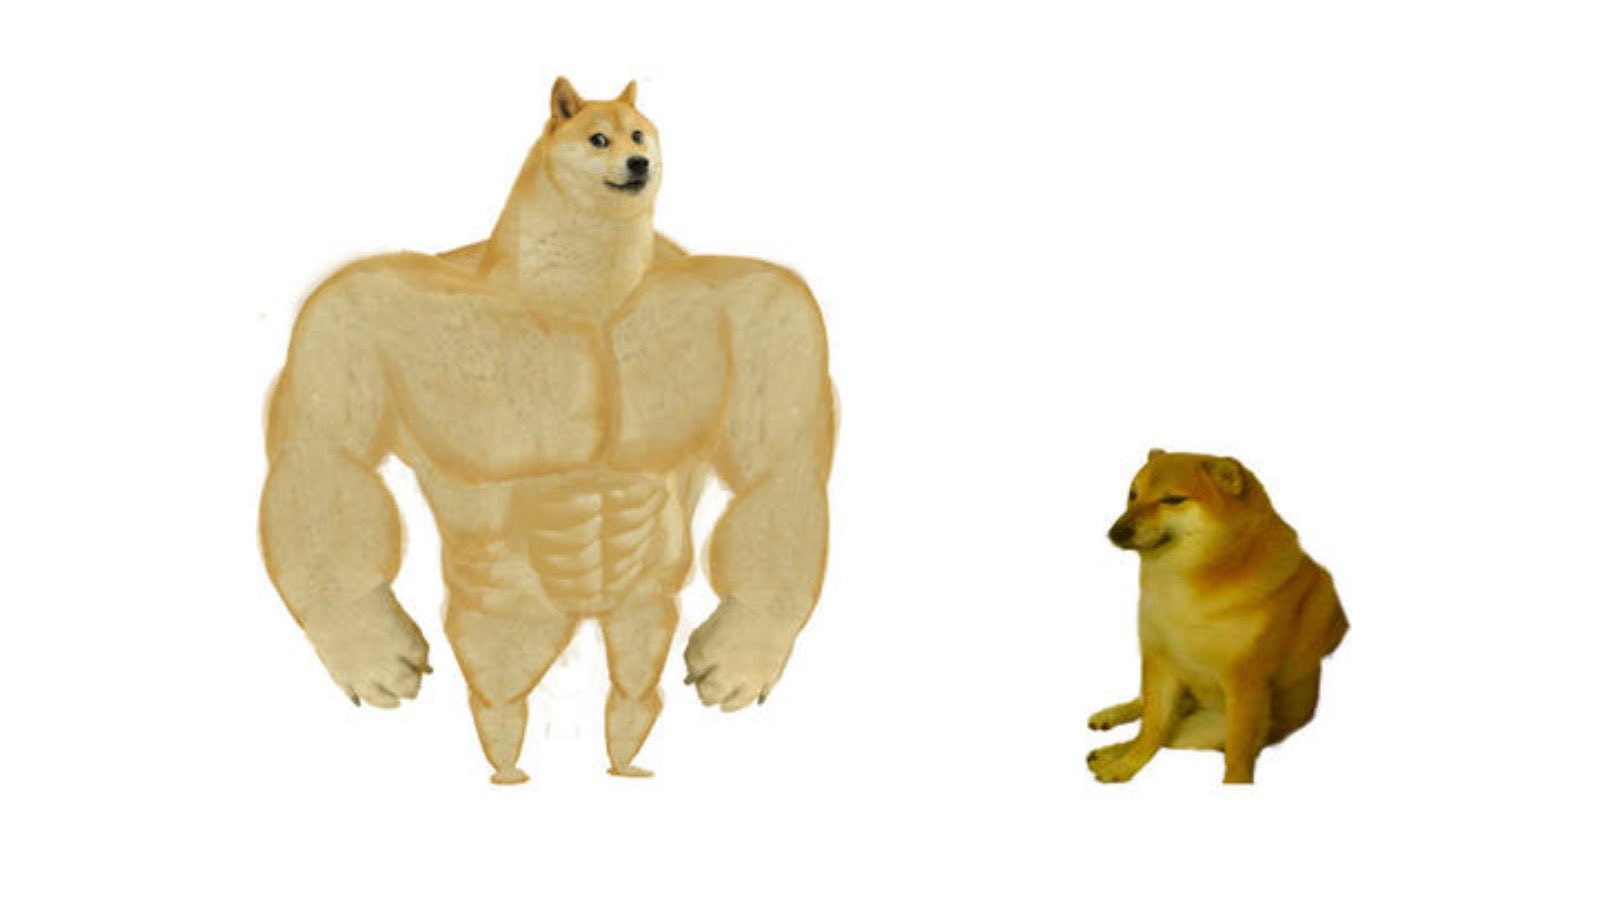
\includegraphics[width=0.4\textwidth]{ChadPython.jpg}
		
	\end{figure}
	\begin{columns}
	\begin{column}{0.7\textwidth}
		Chad Python ist/hat...
		\begin{itemize}
			\item anfängerfreundlich
			\item frei verfügbar
			\item langsam, aber mit Auswegen
			\item sehr gut unterstützt \\(Pakete, StackOverflow Diskussionen, $\dots$)
			\item eine wunderbare Community
			\item verdammt beliebt
		\end{itemize}
	\end{column}
	\begin{column}{0.4\textwidth}
		Andere Programmiersprachen sind...
		\begin{itemize}
			\item kompliziert
			\item teuer
			\item auch langsam
			\item weniger breit anwendbar
			\item unbeliebt
		\end{itemize}
	\end{column}
	\end{columns}
	
\end{frame}

\begin{frame}
	\huge Zeit für Fragen.
\end{frame}


\end{document}